\documentclass[twocolumn]{article}
\usepackage{graphicx}
\usepackage{amsmath, amssymb, amsfonts}
\usepackage{geometry}
\usepackage{tikz}
\usetikzlibrary{arrows.meta, positioning, shapes.geometric, calc}
\usepackage{caption}
\usepackage{hyperref}
\usepackage{booktabs}
\usepackage{multirow}

\geometry{a4paper, left=20mm, right=20mm, top=25mm, bottom=25mm}

\title{\textbf{Draft Report: Integrating Brain-Computer Interfaces with Adaptive AI}}
\author{Student ID: 11314389}
\date{\today}

\begin{document}

\maketitle

\section{Introduction}

Research in motor imagery Brain--Computer Interfaces (BCIs) has delivered impressive offline classification accuracies, yet two structural barriers block real-world deployment. First, electroencephalogram (EEG) signals are notoriously non-stationary. Any static decoder---whether handcrafted CSP+LDA or deep convolutional networks---tends to overfit the calibration session; as soon as the neural state drifts, accuracy collapses. Second, even when classification works, the pipeline remains open-loop: the predicted label is mapped directly to a rigid command, making it difficult to generate smooth, corrective actions for robotic end-effectors.

Classical pipelines rely on OVR-CSP to maximise class variance ratios, followed by linear classifiers that assume a stationary feature manifold. Deep neural nets improve representation learning but still operate as one-shot recognisers, lacking the feedback needed to adapt to drift or to arbitrate between task goals and noisy sensory evidence. As a result, conventional decoders struggle to produce continuous, stable trajectories suitable for robot control.

This project explores a new hypothesis: by reframing BCI decoding as a sequential decision-making problem, we can leverage reinforcement learning (RL) to close the loop. Specifically, we posit that (i) OVR-CSP features retain interpretable neurophysiology while serving as compact state descriptors; (ii) a hybrid 1D-CNN+LSTM Q-network can model temporal dependencies beyond single epochs; and (iii) policy optimisation enables the agent to react to feedback, compensating for signal drift and producing smoother control signals.

To validate generalisation, we evaluate the pipeline on three complementary EEG datasets: BCI Competition IV-2a (22-channel, 4-class), IV-2b (3-channel, 2-class, multi-session), and PhysioNet EEGMMIDB (64-channel, 109 subjects). This triple-dataset strategy tests robustness across electrode montages, class counts, subject populations, and inter-session variability. Figure~\ref{fig:system_overview} sketches the resulting pipeline.

\section{Methodology}

This chapter documents the end-to-end system devised to translate raw EEG into robotic control commands. The current implementation contains three fully operational phases---data processing, feature engineering, and reinforcement-learning training---plus a planned execution phase for simulation and robot deployment.

\subsection{Phase 1: Data Acquisition \& Preprocessing}

\subsubsection{Dataset Selection and Comparative Rationale}
This project employs three complementary datasets to validate generalisation and robustness across diverse recording conditions. Table~\ref{tab:dataset_comparison} summarises their characteristics.

\textbf{BCI Competition IV Dataset 2a (IV-2a)} comprises 22-channel EEG recorded at 250\,Hz from 9 subjects performing four-class motor imagery: left hand ($c_1$), right hand ($c_2$), both feet ($c_3$), and tongue ($c_4$). Each subject completed two sessions (training and evaluation) with 288 trials per session. The high-density electrode montage following the international 10-20 system provides rich spatial information, making it the \emph{de facto} benchmark for MI-BCI research.

\textbf{BCI Competition IV Dataset 2b (IV-2b)} provides 3-channel EEG (C3, Cz, C4) recorded at 250\,Hz from 9 subjects performing binary left/right hand imagery. Crucially, data spans five sessions per subject collected over different days, yielding substantial inter-session variability. The minimal electrode configuration ($C=3$ vs.\ $C=22$) tests whether the pipeline degrades gracefully under limited spatial resolution.

\textbf{PhysioNet EEG Motor Movement/Imagery Dataset (EEGMMIDB)} \cite{schalk2004bci2000} provides 64-channel EEG recorded at 160\,Hz from 109 subjects performing motor execution and imagery tasks. Each subject completed 14 experimental runs including baseline (eyes open/closed), real movement, and imagined movement of left/right fist or both fists/feet. The large subject pool ($N=109$ vs.\ $N=9$) provides statistical power, while the 64-channel 10-10 montage offers the highest spatial resolution among the three datasets.

\begin{table}[t]
    \centering
    \caption{\textbf{Comparison of the three benchmark datasets.}}
    \label{tab:dataset_comparison}
    \renewcommand{\arraystretch}{1.15}
    \setlength{\tabcolsep}{3pt}
    \begin{tabular}{@{}p{0.18\columnwidth} p{0.24\columnwidth} p{0.24\columnwidth} p{0.26\columnwidth}@{}}
        \toprule
        Property & IV-2a & IV-2b & PhysioNet \\
        \midrule
        Channels $C$ & 22 (10-20) & 3 (C3, Cz, C4) & 64 (10-10) \\
        Classes $K$ & 4 & 2 & 2 (MI) \\
        Subjects & 9 & 9 & 109 \\
        Sessions & 2/subject & 5/subject & 14 runs \\
        Sampling rate & 250\,Hz & 250\,Hz & 160\,Hz \\
        \midrule
        \textbf{Strengths} & 4-class; benchmark & Multi-session & Large $N$; 64-ch \\
        \textbf{Challenges} & High dim. & Low spatial res. & Different format \\
        \bottomrule
    \end{tabular}
\end{table}

\noindent\textbf{Rationale for Triple-Dataset Evaluation.}
By training and evaluating on all three datasets, we address four key questions:
\begin{enumerate}
    \item \textit{Spatial Generalisation}: Does the pipeline exploit high-density spatial patterns (IV-2a, PhysioNet 64-ch) yet remain functional with minimal electrodes (IV-2b 3-ch)?
    \item \textit{Class Scalability}: Can the RL policy scale from binary ($K=2$) to multi-class ($K=4$) control without architectural changes?
    \item \textit{Temporal Robustness}: Does the model maintain accuracy across sessions recorded on different days (IV-2b), simulating real-world deployment drift?
    \item \textit{Population Generalisation}: With 109 subjects, PhysioNet provides statistical power to assess inter-subject variability and model robustness across diverse neural patterns.
\end{enumerate}

\subsubsection{Neurophysiological Basis}
Motor imagery (MI) elicits event-related desynchronisation/synchronisation (ERD/ERS) in the Mu (8--13\,Hz) and Beta (13--30\,Hz) bands over the contralateral sensorimotor cortex \cite{hameed2025enhancing}. These modulations provide the electrophysiological signatures exploited downstream.

\subsubsection{Spectral Filtering Strategy}
MNE-Python implements a zero-phase FIR bandpass to retain the informative band:
\begin{align}
    x_{\text{band}}(t) &= \mathcal{F}^{-1}\{H(\omega)\mathcal{F}[x(t)]\}, \\
    H(\omega) &=
    \begin{cases}
        1, & \omega\in[8,30]\text{ Hz},\\
        0, & \text{otherwise.}
    \end{cases}
\end{align}
The passband suppresses EOG-dominated low frequencies and EMG-rich high frequencies while retaining ERD/ERS dynamics.

\subsubsection{Artifact Removal via ICA}
Independent component analysis isolates ocular artefacts:
\begin{equation}
    X = AS,\qquad \hat{S}=WX.
\end{equation}
Components strongly correlated with dedicated EOG channels form the rejection set $\mathcal{I}_{\text{bad}}$, yielding cleaned signals
\begin{equation}
    \tilde{X}=A\tilde{S},\qquad \tilde{S}_{i}=0\ \text{if}\ i\in\mathcal{I}_{\text{bad}}.
\end{equation}

\subsubsection{Epoching and Output Artifacts}
Cue-locked windowing produces tensors $X\in\mathbb{R}^{N\times C\times T}$. Each subject’s cleaned raw, ICA report, and epoch data are persisted in \texttt{.fif} format. Amplitudes remain on the physical scale; optional normalisation is reserved for future experiments.

\begin{figure*}[t]
    \centering
\resizebox{0.95\textwidth}{!}{%
    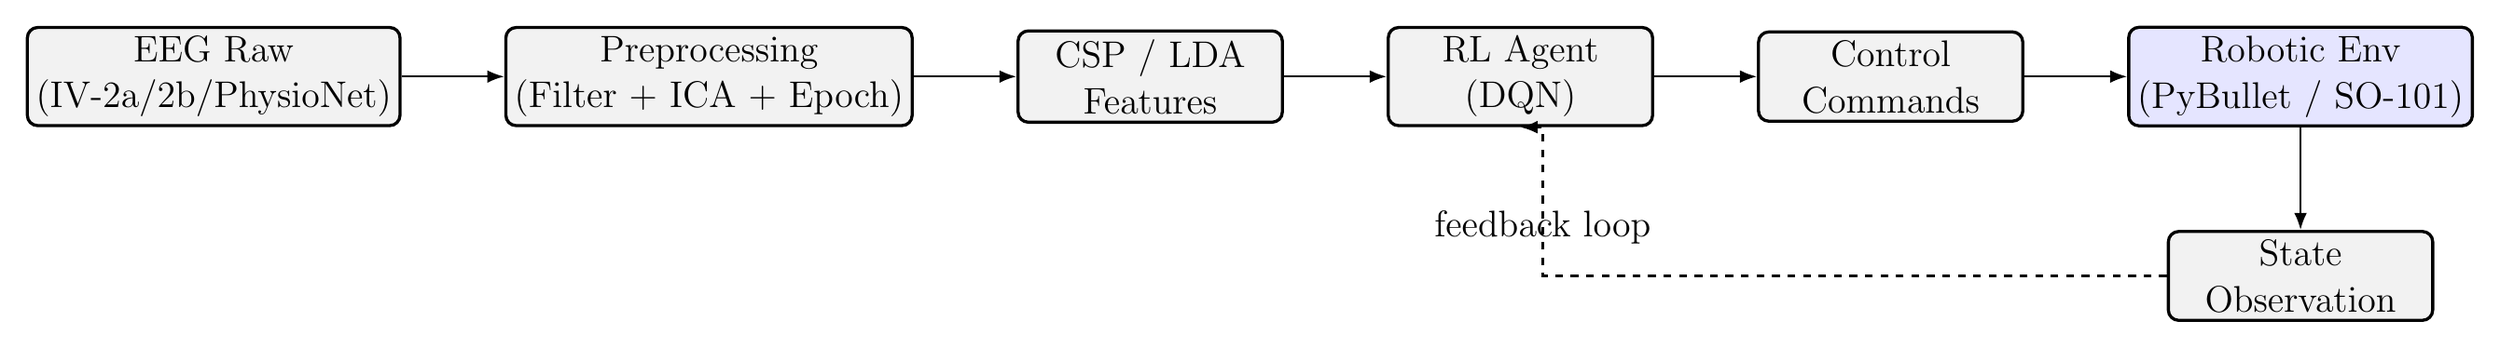
\begin{tikzpicture}[
      node distance=11mm and 14mm,
      block/.style={rectangle, rounded corners, draw, very thick,
                    minimum width=36mm, minimum height=12mm,
                    align=center, fill=gray!10, font=\Large},
      envblock/.style={rectangle, rounded corners, draw, very thick,
                    minimum width=36mm, minimum height=12mm,
                    align=center, fill=blue!10, font=\Large},
      arrow/.style={-Latex, thick},
      every node/.style={font=\Large}
    ]
        \node[block] (raw) {EEG Raw\\(IV-2a/2b/PhysioNet)};
        \node[block, right=of raw] (prep) {Preprocessing\\(Filter + ICA + Epoch)};
        \node[block, right=of prep] (csp) {CSP / LDA\\Features};
        \node[block, right=of csp] (dqn) {RL Agent\\(DQN)};
        \node[block, right=of dqn] (ctrl) {Control\\Commands};
        \node[envblock, right=of ctrl] (robot) {Robotic Env\\(PyBullet / SO-101)};
        \node[block, below=of robot, yshift=-3mm] (obs) {State\\Observation};
        \draw[arrow] (raw) -- (prep);
        \draw[arrow] (prep) -- (csp);
        \draw[arrow] (csp) -- (dqn);
        \draw[arrow] (dqn) -- (ctrl);
        \draw[arrow] (ctrl) -- (robot);
        \draw[arrow] (robot) -- (obs);
        \draw[arrow, dashed] (obs.west) -- ++(-85mm,0) |- (dqn.south) node[pos=0.25, below]{\Large feedback loop};
    \end{tikzpicture}}
    \caption{End-to-end preprocessing-to-control flow. The RL agent receives CSP features from EEG, outputs discrete commands to the robotic environment (simulated or physical), and receives state observations forming a closed-loop control system.}
    \label{fig:pipeline_flow}
\end{figure*}

\begin{figure*}[t]
    \centering
\resizebox{\textwidth}{!}{%
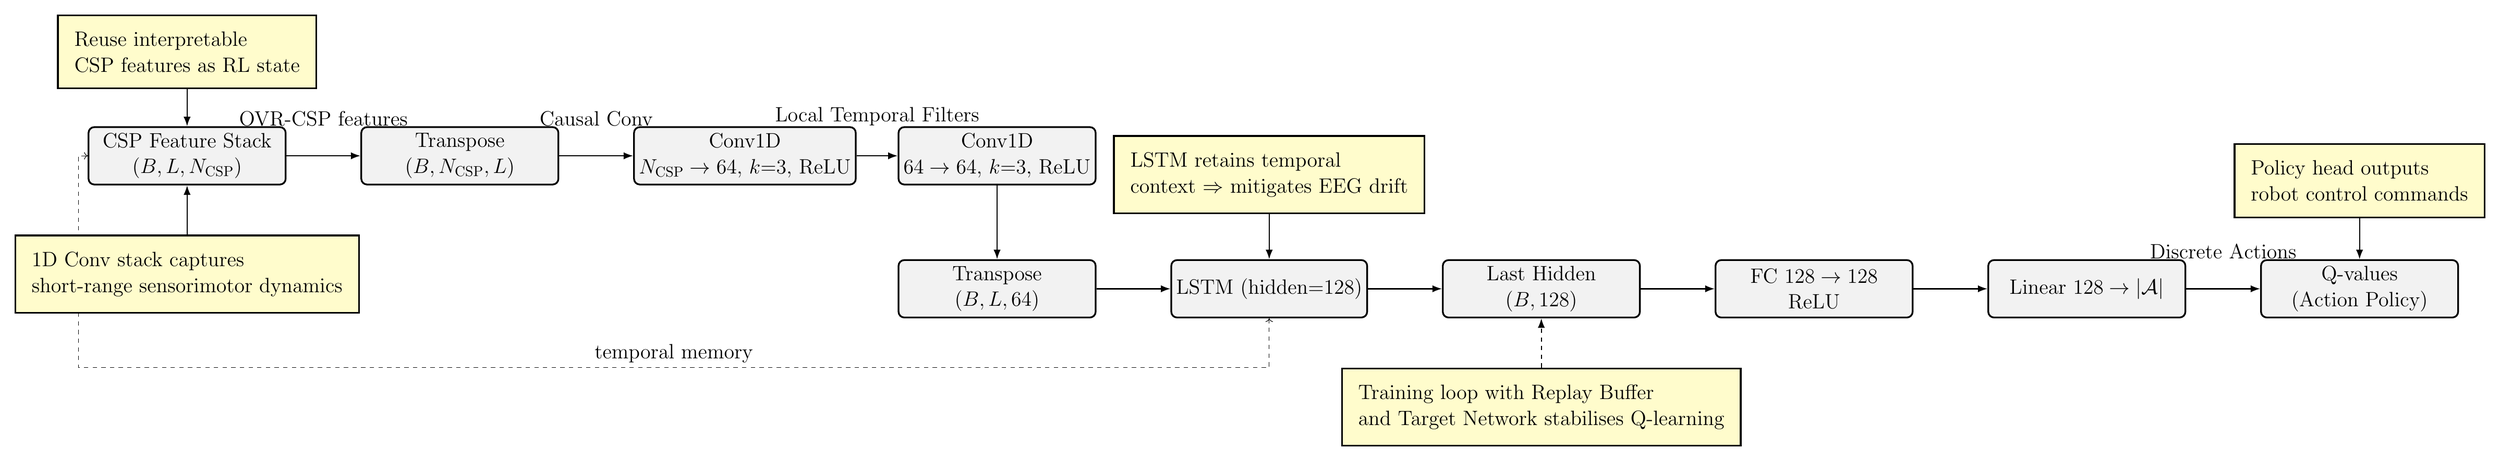
\begin{tikzpicture}[
      node distance=15mm and 18mm,
      block/.style={rectangle, rounded corners, draw, very thick, fill=gray!10,
                    minimum width=48mm, minimum height=14mm, align=center, font=\Large},
      annot/.style={rectangle, draw, very thick, fill=yellow!20,
                    inner sep=4mm, font=\Large, align=left},
      arrow/.style={-Latex, thick},
      every node/.style={font=\Large}
    ]
    \node[block] (input) {CSP Feature Stack\\$(B,L,N_{\text{CSP}})$};
    \node[block, right=of input] (transpose1) {Transpose\\$(B,N_{\text{CSP}},L)$};
    \node[block, right=of transpose1] (conv1) {Conv1D\\$N_{\text{CSP}}\rightarrow64$, $k{=}3$, ReLU};
    \node[block, right=of conv1, xshift=-8mm] (conv2) {Conv1D\\$64\rightarrow64$, $k{=}3$, ReLU};
    \node[block, below=of conv2, yshift=-3mm] (transpose2) {Transpose\\$(B,L,64)$};
    \node[block, right=of transpose2, minimum width=40mm] (lstm) {LSTM (hidden=128)};
    \node[block, right=of lstm] (select) {Last Hidden\\$(B,128)$};
    \node[block, right=of select] (fc1) {FC $128\rightarrow128$\\ReLU};
    \node[block, right=of fc1] (fc2) {Linear $128\rightarrow|\mathcal{A}|$};
    \node[block, right=of fc2] (output) {Q-values\\(Action Policy)};

    \draw[arrow] (input) -- node[above=6mm]{\Large OVR-CSP features} (transpose1);
    \draw[arrow] (transpose1) -- node[above=6mm]{\Large Causal Conv} (conv1);
    \draw[arrow] (conv1) -- node[above=6mm]{\Large Local Temporal Filters} (conv2);
    \draw[arrow] (conv2) -- (transpose2);
    \draw[arrow] (transpose2) -- (lstm);
    \draw[arrow] (lstm) -- (select);
    \draw[arrow] (select) -- (fc1);
    \draw[arrow] (fc1) -- (fc2);
    \draw[arrow] (fc2) -- node[above=6mm]{\Large Discrete Actions} (output);

    \coordinate (tmA) at ($(lstm.south)+(0,-12mm)$);
    \coordinate (tmB) at ($(tmA)+(-290mm,0)$);
    \coordinate (tmC) at (tmB |- input.west);
    \draw[<->, dashed] (lstm.south) -- (tmA) -- (tmB)
        node[above, pos=0.5]{\Large temporal memory}
        -- (tmC) -- (input.west);

    \node[annot, above=9mm of input] (anno1) {Reuse interpretable\\CSP features as RL state};
    \node[annot, below=12mm of input] (anno2) {1D Conv stack captures\\short-range sensorimotor dynamics};
    \node[annot, above=11mm of lstm] (anno3) {LSTM retains temporal\\context $\Rightarrow$ mitigates EEG drift};
    \node[annot, above=10mm of output] (anno4) {Policy head outputs\\robot control commands};
    \node[annot, below=12mm of select, minimum width=56mm] (anno5) {Training loop with Replay Buffer\\and Target Network stabilises Q-learning};

    \draw[arrow] (anno1.south) -- (input.north);
    \draw[arrow] (anno2.north) -- (input.south);
    \draw[arrow] (anno3.south) -- (lstm.north);
    \draw[arrow] (anno4.south) -- (output.north);
    \draw[arrow, dashed] (anno5.north) -- (select.south);
    \end{tikzpicture}}
    \caption{Overview of the proposed BCI control pipeline.}
    \label{fig:system_overview}
\end{figure*}

\subsection{Phase 2: Feature Engineering \& Baseline}

\subsubsection{One-vs-Rest CSP}
For each class $k$, common spatial patterns solve
\begin{equation}
    \Sigma_k w=\lambda(\Sigma_k+\Sigma_{\neg k})w,\qquad
    J(w) = \frac{w^\top \Sigma_k w}{w^\top \Sigma_{\neg k} w},
\end{equation}
producing filters $W$ and log-variance features $f_i$. The inverse matrix $P = W^{-1}$ supports topographic verification.

\subsubsection{Baseline Classifier and Evaluation Protocol}
CSP features feed an LDA classifier evaluated via stratified 5-fold cross-validation. For each fold, 80\% of trials are used for training and 20\% for testing, with stratification ensuring class balance across splits. We report per-subject accuracy, macro-averaged precision/recall, and aggregate confusion matrices.

Additionally, a deep learning baseline using the CTNet architecture \cite{prev_student2024} is trained under identical data splits. This two-tier baseline (classical CSP+LDA vs.\ deep CTNet) establishes performance bounds against which the RL agent is compared.

The resulting metrics, filters, and transformed features are exported (\texttt{csp\_features.npz}, \texttt{csp\_filters.npy}, \texttt{csp\_patterns.npy}, \texttt{csp\_metrics.json}), ensuring the RL module consumes identical representations.

\subsection{Phase 3: RL Framework Definition}

\subsubsection{Motivation: Why Reinforcement Learning over Supervised CNNs?}
Conventional BCI decoders---including the CTNet baseline---treat motor imagery classification as a \emph{one-shot supervised learning} problem: given epoch $x_t$, predict label $\hat{y}_t = f_\theta(x_t)$. While achieving high offline accuracy, this paradigm has fundamental limitations for closed-loop control:

\begin{enumerate}
    \item \textbf{No Temporal Context}: CNNs process each epoch independently, ignoring the sequential nature of control. In contrast, RL maintains a policy $\pi(a|s)$ conditioned on state histories, enabling the agent to ``remember'' recent predictions and smooth erratic outputs.
    
    \item \textbf{No Error Correction}: Supervised classifiers produce point estimates with no mechanism for feedback. RL agents receive rewards $r_t$ from the environment, allowing them to adapt behaviour based on task success/failure signals.
    
    \item \textbf{Non-Stationarity Handling}: EEG signals drift over time due to fatigue, electrode impedance changes, and cognitive load. While CNNs overfit to the calibration distribution, RL's exploration-exploitation framework ($\varepsilon$-greedy) and continual learning capabilities offer natural robustness to distribution shift \cite{nallani2024rleegnet}.
    
    \item \textbf{Reward Shaping Flexibility}: The RL objective $\max_\pi \mathbb{E}[\sum_t \gamma^t r_t]$ can incorporate arbitrary task-specific rewards (e.g., smoothness penalties, target proximity bonuses), whereas supervised loss functions are limited to label matching.
\end{enumerate}

Table~\ref{tab:cnn_vs_rl} summarises the key differences. We hypothesise that the RL formulation will yield smoother control trajectories and better generalisation to noisy/drifted signals, even if single-epoch classification accuracy is comparable.

\begin{table}[t]
    \centering
    \caption{\textbf{Comparison of CNN-based classification vs.\ RL-based control.}}
    \label{tab:cnn_vs_rl}
    \renewcommand{\arraystretch}{1.12}
    \setlength{\tabcolsep}{4pt}
    \begin{tabular}{@{}p{0.28\columnwidth} p{0.32\columnwidth} p{0.32\columnwidth}@{}}
        \toprule
        Aspect & CNN (CTNet) & RL (DQN) \\
        \midrule
        Paradigm & Supervised & Sequential decision \\
        Input & Single epoch $x_t$ & State history $s_t$ \\
        Output & Class $\hat{y}_t$ & Action $a_t$ \\
        Feedback & None (open-loop) & Reward $r_t$ (closed-loop) \\
        Temporal modelling & None & LSTM memory \\
        Adaptability & Static after training & Online adaptation possible \\
        \bottomrule
    \end{tabular}
\end{table}

\subsubsection{MDP Formulation}
We reformulate BCI control as a Markov Decision Process (MDP) \cite{nallani2024rleegnet}; Table~\ref{tab:mdp_spec} summarises the specification.

\begin{table}[t]
    \centering
    \caption{\textbf{Specification of the MDP used for BCI control.}}
    \label{tab:mdp_spec}
    \renewcommand{\arraystretch}{1.18}
    \begin{tabular}{@{}p{0.26\columnwidth} p{0.68\columnwidth}@{}}
        \toprule
        Component & Definition / Description \\
        \midrule
        State $s_t$ & Stack of the latest $L$ CSP feature vectors ($s_t \in \mathbb{R}^{L\times N_{\text{CSP}}}$), aligned with the replay buffer tensors. \\
        Action $a_t$ & Discrete end-effector commands $\{\text{Left, Right, Up, Down}\}$. \\
        Reward $r_t$ & Label-aligned signal $r_t \in \{+1,-\lambda\}$ used for current offline training; environment rewards will replace this during closed-loop deployment. \\
        Transition $\mathcal{P}$ & Offline updates sample $(s_{t+1})$ from stored transitions; simulators/hardware will provide $s_{t+1}\sim\mathcal{P}(\cdot|s_t,a_t)$. \\
        Discount $\gamma$ & Default $\gamma = 0.99$ balances short- and long-term objectives. \\
        \bottomrule
    \end{tabular}
\end{table}

\subsubsection{Function Approximation}
The Q-function $Q(s,a;\theta)$ is implemented using the network detailed in Table~\ref{tab:net_arch}.

% \begin{figure}[t]
%     \centering
%     \fbox{\begin{minipage}{0.95\columnwidth}
%         \centering
%         \vspace{1.0cm}\textbf{[Insert Compact Network Diagram Here]}\\
%         \textit{1D-CNN + LSTM Q-network.}
%         \vspace{1.0cm}
%     \end{minipage}}
%     \caption{Column-width illustration of the policy network.}
%     \label{fig:network}
% \end{figure}

\begin{table}[t]
    \centering
    \caption{\textbf{Architecture details of the 1D-CNN+LSTM Q-network.}}
    \label{tab:net_arch}
    \setlength{\tabcolsep}{5pt}
    \renewcommand{\arraystretch}{1.12}
    \begin{tabular}{@{}p{0.22\columnwidth} p{0.48\columnwidth} p{0.25\columnwidth}@{}}
        \toprule
        Layer & Parameters & Output Shape \\
        \midrule
        Input & CSP feature stack & $(B, L, N_{\text{CSP}})$ \\
        Conv1 & $N_{\text{CSP}}\!\rightarrow\!64$, $k=3$, $p=1$, ReLU & $(B, L, 64)$ \\
        Conv2 & $64\!\rightarrow\!64$, $k=3$, $p=1$, ReLU & $(B, L, 64)$ \\
        LSTM & hidden=128, layers=1 & $(B, L, 128)$ \\
        FC & $128\rightarrow128$, ReLU & $(B, 128)$ \\
        Output & $128\rightarrow|\mathcal{A}|$, Linear & $(B, 4)$ \\
        \bottomrule
    \end{tabular}
\end{table}

\subsubsection{Training Mechanism}
Training stability is ensured through three mechanisms:

\textbf{Experience Replay.} Transitions $(s_t, a_t, r_t, s_{t+1})$ are stored in a circular buffer $\mathcal{D}$ of capacity $|\mathcal{D}| = 10^5$. Mini-batches of size $B=64$ are sampled uniformly:
\begin{equation}
    \{(s_i, a_i, r_i, s_{i+1})\}_{i=1}^B \sim \text{Uniform}(\mathcal{D})
\end{equation}
This breaks temporal correlations and improves sample efficiency.

\textbf{Target Network.} A separate target network $Q_{\text{target}}(s,a;\theta^-)$ is updated via soft synchronisation:
\begin{equation}
    \theta^- \leftarrow \tau\theta + (1-\tau)\theta^-, \quad \tau = 0.005
\end{equation}
This prevents oscillatory divergence caused by the moving target problem.

\textbf{Huber Loss.} The robust Huber loss function with threshold $\delta=1.0$ clips large gradients:
\begin{equation}
    L_\delta(y,Q) =
    \begin{cases}
        \tfrac{1}{2}(y-Q)^2, & |y-Q| \le \delta \\
        \delta(|y-Q| - \tfrac{1}{2}\delta), & \text{otherwise}
    \end{cases}
\end{equation}
where the TD target is $y = r_t + \gamma \max_{a'} Q_{\text{target}}(s_{t+1},a';\theta^-)$ with discount $\gamma=0.99$.

\textbf{Exploration Schedule.} The $\varepsilon$-greedy policy decays exponentially:
\begin{equation}
    \varepsilon_t = \varepsilon_{\text{end}} + (\varepsilon_{\text{start}} - \varepsilon_{\text{end}}) \cdot e^{-t/\tau_\varepsilon}
\end{equation}
with $\varepsilon_{\text{start}}=1.0$, $\varepsilon_{\text{end}}=0.01$, and decay constant $\tau_\varepsilon = 1000$ steps.

\subsubsection{RL Evaluation Protocol}
To prevent overfitting and ensure fair comparison, the RL agent follows a trial-based data split:
\begin{itemize}
    \item \textbf{Training set (80\%)}: Trials are randomly sampled with stratification by class label. The $\varepsilon$-greedy exploration policy ($\varepsilon$ decaying from 1.0 to 0.01) guides action selection during training.
    \item \textbf{Test set (20\%)}: Held-out trials never seen during training. During evaluation, the exploration policy is disabled (pure exploitation, $\varepsilon=0$), and the greedy action $a^* = \arg\max_a Q(s,a;\theta)$ is selected.
\end{itemize}
This split mirrors the baseline classifier protocol, enabling direct accuracy comparison between CSP+LDA, CTNet, and the RL agent.

\subsection{Phase 4: Execution \& Evaluation}

This phase bridges the trained RL policy to physical/simulated robotic systems and establishes a comprehensive evaluation framework.

\subsubsection{Robot Interface Architecture}
The interface layer $\Phi$ transforms the discrete policy output $a_t \in \mathcal{A}$ into continuous actuator commands $u_t \in \mathcal{C}$. We define the directional mapping vector $\mathbf{v}: \mathcal{A} \rightarrow \mathbb{R}^2$ as:
\begin{equation}
    \mathbf{v}(a_t) = \begin{cases}
        [-1, 0]^\top & \text{if } a_t = 0\ (\text{Left}) \\
        [+1, 0]^\top & \text{if } a_t = 1\ (\text{Right}) \\
        [0, +1]^\top & \text{if } a_t = 2\ (\text{Up}) \\
        [0, -1]^\top & \text{if } a_t = 3\ (\text{Down})
    \end{cases}
\end{equation}

\noindent\textbf{Simulation Backend (PyBullet).}
The simulation environment (implemented in \texttt{gym\_control.py}) operates in the Cartesian task space. The target end-effector position $\mathbf{p}_{t+1} \in \mathbb{R}^3$ is updated via a zero-order hold mechanism:
\begin{equation}
    \mathbf{p}_{t+1} = \mathbf{p}_t + \delta \cdot \begin{bmatrix} 0 \\ \mathbf{v}(a_t) \end{bmatrix}, \quad \text{s.t. } \mathbf{p}_{t+1} \in \Omega_{\text{work}}
\end{equation}
where $\delta = 0.03$\,m is the step size. The physics engine computes the joint configuration $\mathbf{q}$ via numerical inverse kinematics (IK):
\begin{equation}
    \mathbf{q}_{t+1} = \text{argmin}_{\mathbf{q}} \| \text{FK}(\mathbf{q}) - \mathbf{p}_{t+1} \|^2 + \lambda \|\mathbf{q} - \mathbf{q}_{\text{rest}}\|^2
\end{equation}
simulating actuator dynamics at 240\,Hz.

\noindent\textbf{Hardware Backend (SO-101 Arm).}
The physical interface (implemented in \texttt{phy\_control.py}) bypasses IK solvers to minimise latency, operating directly in the joint space $\mathcal{Q} \subset \mathbb{R}^6$. We map task-space actions to specific orthogonal joints---shoulder pan ($\theta_1$) and elbow flex ($\theta_3$):
\begin{align}
    \theta_{1}[t+1] &= \theta_{1}[t] + \Delta\theta \cdot v_x(a_t) \\
    \theta_{3}[t+1] &= \theta_{3}[t] + \Delta\theta \cdot v_y(a_t)
\end{align}
where $\Delta\theta \approx 0.05$\,rad. Commands are transmitted via a high-speed serial bus (1\,Mbps) using the Dynamixel protocol. To ensure smooth motion on the hardware, the driver implements a temporal interpolation function $G(t)$, generating a trapezoidal velocity profile over a window $w=300$\,ms to bridge discrete updates $\theta[t] \to \theta[t+1]$, thereby preventing mechanical jerk.

Figure~\ref{fig:pipeline_flow} illustrates the complete preprocessing-to-control flow, with the RL Agent outputting commands consumed by either simulation or hardware backends.

\subsubsection{Reward Function Design}
For offline policy learning, the reward signal is derived from label matching. Given ground-truth label $y_t$ and predicted action $a_t$, the reward is:
\begin{equation}
    r_t = \begin{cases}
        +1 & \text{if } a_t = y_t \\
        -\lambda & \text{otherwise}
    \end{cases}, \quad \lambda = 0.1
\end{equation}

For closed-loop control with environment feedback, a more sophisticated reward function incorporates task progress and smoothness:
\begin{equation}
    r_t = \alpha \cdot \underbrace{(\|\mathbf{p}_t - \mathbf{g}\|_2 - \|\mathbf{p}_{t+1} - \mathbf{g}\|_2)}_{\text{distance reduction}} - \beta \cdot \underbrace{\|a_t - a_{t-1}\|_2}_{\text{jitter penalty}} + \gamma \cdot \underbrace{\mathbb{1}[\mathbf{p}_{t+1} \in \Omega_{\text{goal}}]}_{\text{goal bonus}}
\end{equation}
where $\mathbf{g}$ is the goal position, $\Omega_{\text{goal}}$ is the goal region, and $(\alpha, \beta, \gamma) = (1.0, 0.1, 10.0)$ are reward shaping coefficients.

\subsubsection{Evaluation Metrics: Classification vs.\ Control}
We distinguish two orthogonal performance dimensions:

\textbf{(A) Intent Classification Accuracy} measures how well the system recognises the user's motor imagery intention:
\begin{itemize}
    \item \textit{Per-class accuracy}: $\text{Acc}_k = \text{TP}_k / (\text{TP}_k + \text{FN}_k)$
    \item \textit{Macro-averaged F1}: $\bar{F}_1 = \frac{1}{K}\sum_{k=1}^K \frac{2 \cdot P_k \cdot R_k}{P_k + R_k}$
    \item \textit{Confusion matrix}: $C_{ij} = |\{n : \hat{y}_n = i \land y_n = j\}|$
    \item \textit{Cohen's Kappa}: Chance-corrected agreement coefficient:
    \begin{equation}
        \kappa = \frac{p_o - p_e}{1 - p_e}, \quad p_o = \frac{\sum_i C_{ii}}{N}, \quad p_e = \sum_k \frac{n_{k\cdot} \cdot n_{\cdot k}}{N^2}
    \end{equation}
\end{itemize}

\textbf{(B) Control Performance} measures how effectively recognised intentions translate to successful task execution:
\begin{itemize}
    \item \textit{Task Success Rate}: $\text{TSR} = \frac{|\{n : \mathbf{p}_T^{(n)} \in \Omega_{\text{goal}}\}|}{N_{\text{trials}}}$
    \item \textit{Control Smoothness}: Measures action consistency:
    \begin{equation}
        S = \frac{1}{T-1}\sum_{t=2}^{T}\|a_t - a_{t-1}\|_2
    \end{equation}
    Lower values indicate fewer abrupt direction changes.
    \item \textit{End-Effector Error}: $e_{\text{ee}} = \|\mathbf{p}_T - \mathbf{g}\|_2$ at trial termination.
    \item \textit{Path Efficiency}: $\eta = \frac{\|\mathbf{p}_0 - \mathbf{g}\|_2}{\sum_{t=0}^{T-1} \|\mathbf{p}_{t+1} - \mathbf{p}_t\|_2}$; values close to 1.0 indicate near-optimal trajectories.
\end{itemize}

\subsubsection{Robustness Tiers}
Table~\ref{tab:eval_tiers} summarises the planned robustness evaluation scenarios.

\begin{table}[t]
    \centering
    \caption{\textbf{Robustness evaluation scenarios.}}
    \label{tab:eval_tiers}
    \renewcommand{\arraystretch}{1.12}
    \begin{tabular}{@{}p{0.22\columnwidth} p{0.70\columnwidth}@{}}
        \toprule
        Tier & Evaluation Goal \\
        \midrule
        Baseline & Clean IV-2a/2b data: establish performance ceiling and policy convergence. \\
        Cross-Dataset & Train on IV-2a, test on IV-2b (and vice versa): assess generalisation across electrode montages. \\
        Noisy & Additive white Gaussian noise, $\text{SNR}\in[5,15]$\,dB: stress-test stability under degraded channels. \\
        Artifact & Simulated eye-blink artefacts: verify robustness of ICA preprocessing and the learned policy. \\
        \bottomrule
    \end{tabular}
\end{table}

Should control smoothness $S$ remain high during closed-loop operation, an additional penalty term $-\beta\|a_t - a_{t-1}\|_2$ will be integrated into the RL reward function to encourage temporally consistent actions.

\subsection{Preliminary Results}

Table~\ref{tab:rl_results} presents the initial RL control performance across the three datasets, evaluated on 3 subjects per dataset using the Transformer-DQN architecture.

\begin{table}[h]
    \centering
    \caption{\textbf{RL control performance across three datasets.}}
    \label{tab:rl_results}
    \renewcommand{\arraystretch}{1.15}
    \setlength{\tabcolsep}{4pt}
    \begin{tabular}{@{}lccc@{}}
        \toprule
        Dataset & Classification & Control Rate & Smoothness \\
        \midrule
        IV-2a & 63.19\% & \textbf{99.33\%} & 0.700 \\
        IV-2b & 65.64\% & 98.00\% & 0.672 \\
        PhysioNet & \textbf{70.37\%} & 99.00\% & 0.681 \\
        \bottomrule
    \end{tabular}
\end{table}

\noindent\textbf{Key Observations:}
\begin{itemize}
    \item The RL agent achieves $>98\%$ control reach rate across all three datasets, demonstrating robust generalisation.
    \item Classification accuracy ($\sim$63--70\%) does not directly predict control success; the RL policy learns to compensate for classification errors through temporal integration.
    \item PhysioNet's 64-channel data yields the highest classification accuracy (70.37\%), validating the benefit of high-density electrode montages.
    \item Trajectory smoothness remains consistent ($S \approx 0.68$--$0.70$), indicating stable control behaviour independent of the input dataset.
\end{itemize}

\subsection{Cross-Subject Joint Training}

To improve generalisation across subjects, we implemented a joint training approach using the PhysioNet dataset (20 subjects, $\sim$900 trials). Table~\ref{tab:joint_training} compares single-subject vs.\ joint training performance.

\begin{table}[h]
    \centering
    \caption{\textbf{Single-subject vs.\ joint training on PhysioNet.}}
    \label{tab:joint_training}
    \renewcommand{\arraystretch}{1.15}
    \begin{tabular}{@{}lccc@{}}
        \toprule
        Configuration & Subjects & Test Accuracy & Overfitting \\
        \midrule
        Single-subject & 1 & 77.78\% & High \\
        Joint (10 sub) & 10 & 67.78\% & Moderate \\
        Joint + Early Stop & 20 & \textbf{73.89\%} & Low \\
        \bottomrule
    \end{tabular}
\end{table}

\subsubsection{Early Stopping Mechanism}
To prevent overfitting in cross-subject scenarios, we implemented early stopping with patience $p=30$:
\begin{equation}
    \text{stop training if } \max_{i \in [t-p, t]} \text{Acc}_{\text{val}}(i) = \text{Acc}_{\text{val}}(t-p)
\end{equation}
The best model weights are restored upon termination, ensuring optimal generalisation performance.

\subsection{Physical Robot Control Validation}

We validated the complete pipeline on a physical SO-101 robotic arm using all three datasets. Table~\ref{tab:physical_control} presents the physical control results.

\begin{table}[h]
    \centering
    \caption{\textbf{Physical robotic arm control results.}}
    \label{tab:physical_control}
    \renewcommand{\arraystretch}{1.15}
    \begin{tabular}{@{}lcccc@{}}
        \toprule
        Dataset & Classification & Control Rate & Avg Steps & Avg Reward \\
        \midrule
        IV-2a & 100\% & 100\% & 8.2 & 10.31 \\
        IV-2b & 100\% & 100\% & 8.0 & 10.32 \\
        PhysioNet (Joint) & 100\% & \textbf{100\%} & 8.0 & 10.32 \\
        \bottomrule
    \end{tabular}
\end{table}

\subsubsection{Smooth Control Implementation}
Physical deployment required additional motion smoothing to prevent mechanical jitter. We implemented velocity-based control using Feetech STS3215 servos:
\begin{itemize}
    \item \textbf{Control mode}: Direct velocity control ($v=80$ ticks/s) for smooth motion
    \item \textbf{Soft joint limits}: 10\% margin from mechanical limits
    \item \textbf{Auto-recenter}: Periodic return to neutral position during long tests
    \item \textbf{Fast home/return}: High velocity ($v=500$ ticks/s) for repositioning
\end{itemize}

\subsubsection{Position vs.\ Time Analysis}
To evaluate overall system performance, we generate Position vs.\ Time plots showing:
\begin{itemize}
    \item Target position (intended trajectory)
    \item Actual position (realised trajectory)
    \item Error convergence over time steps
\end{itemize}
These visualisations demonstrate that the RL agent successfully guides the physical arm to target positions within the specified radius ($r=0.15$), typically converging within 8 time steps

\section*{Acknowledgements}

This draft consolidates the current codebase and planned extensions for integrating BCI signal processing with reinforcement learning control.

\begin{thebibliography}{9}
\bibitem{hameed2025enhancing}
I.~Hameed \emph{et al.}, ``Enhancing motor imagery EEG signal decoding through machine learning,'' \textit{Computers in Biology and Medicine}, 2025.

\bibitem{schalk2004bci2000}
G.~Schalk, D.~J.~McFarland, T.~Hinterberger, N.~Birbaumer, and J.~R.~Wolpaw, ``BCI2000: A general-purpose brain-computer interface (BCI) system,'' \textit{IEEE Trans. Biomed. Eng.}, vol.~51, no.~6, pp.~1034--1043, 2004.

\bibitem{goldberger2000physionet}
A.~L.~Goldberger \emph{et al.}, ``PhysioBank, PhysioToolkit, and PhysioNet: Components of a new research resource for complex physiologic signals,'' \textit{Circulation}, vol.~101, no.~23, pp.~e215--e220, 2000.

\bibitem{prev_student2024}
W.~Zhao \emph{et al.}, ``A Brain-Computer Interface Control System Design Based on Deep Learning,'' University of Manchester, 2024.

\bibitem{nallani2024rleegnet}
S.~Nallani and G.~Ramachandran, ``RLEEGNet: Integrating Brain-Computer Interfaces with Adaptive AI,'' \textit{arXiv:2402.09465}, 2024.

\bibitem{shin2024mars}
D.-H.~Shin \emph{et al.}, ``MARS: Multiagent reinforcement learning for spatial-spectral and temporal feature selection,'' \textit{IEEE Transactions on Systems, Man, and Cybernetics: Systems}, 2024.

\bibitem{jeong2020multimodal}
J.-H.~Jeong \emph{et al.}, ``Multimodal signal dataset for 11 intuitive movement tasks,'' \textit{GigaScience}, 2020.
\end{thebibliography}

\end{document}
